
Now that we have our algorithm implemented the one thing left to do is to test it on multiple data sets. This process is very important, because it gives an objective image of what our model is capable of. As for the data sets, we are going to be using those provided in the task.

Since we are not given any information about the age of attendants, to prevent biased results we assumed their age to be the same and equal to a 45, a standard middle age of a human.

\subsection{Scenario 1) "Small Meeting"}

Time: mid-June

Participants:
\begin{itemize}[noitemsep,topsep=0pt,parsep=0pt,partopsep=0pt]
\item Monterey CA, USA
\item Zutphen, Netherlands
\item Melbourne, Australia
\item Shanghai, China
\item Hong Kong (SAR), China
\item Moscow, Russia
\end{itemize}

Screenshot (Figure \ref{res:1}):

\begin{figure}[ht]
    \centering
        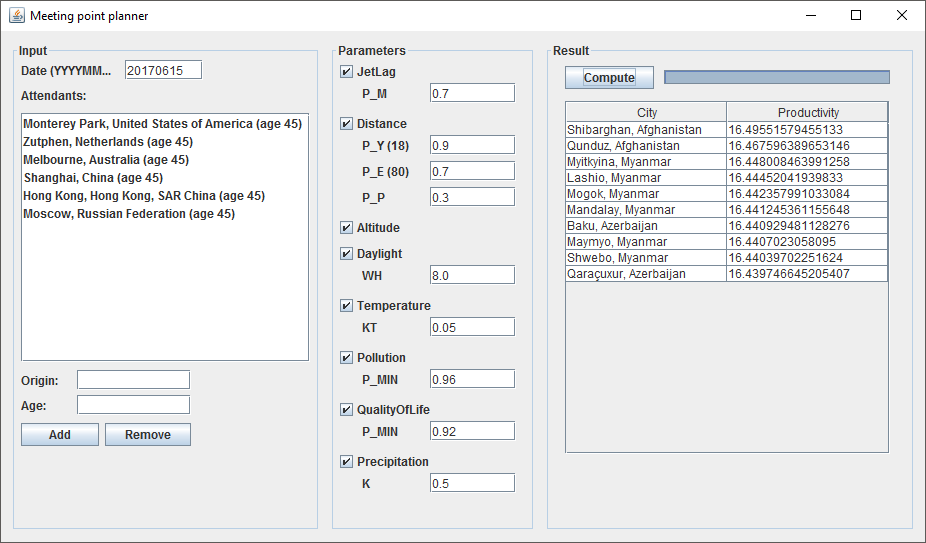
\includegraphics[width=\textwidth]{screenshot1}
    \caption{Results for scenario 1}
    \label{res:1}
\end{figure}

\subsection{Scenario 2) "Big meeting"}

Time: January

Participants:
\begin{itemize}[noitemsep,topsep=0pt,parsep=0pt,partopsep=0pt]
\item Boston MA, USA (2 people)
\item Singapore
\item Beijing, China
\item Hong Kong (SAR), China (2 people)
\item Moscow, Russia
\item Utrecht, Netherlands
\item Warsaw, Poland
\item Copenhagen, Denmark
\item Melbourne, Australia
\end{itemize}

Screenshot (Figure \ref{res:2}):

\begin{figure}[ht]
    \centering
        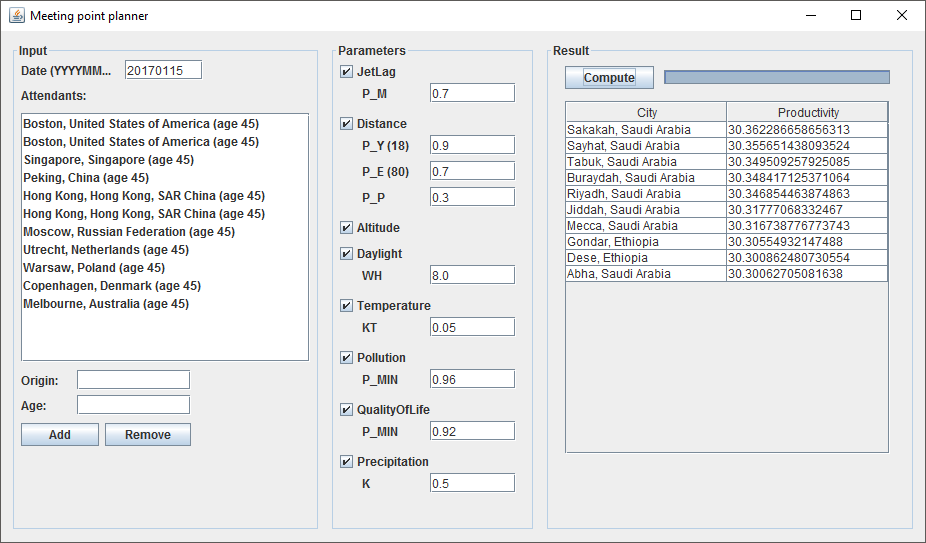
\includegraphics[width=\textwidth]{screenshot2}
    \caption{Results for scenario 2}
    \label{res:2}
\end{figure}


It is important to note that the result highly depends on the parameters that were chosen by us and would normally be set to reflect the basic behavior of people.
